\begin{table}[h]
	\centering
	\begin{tabular}{|c||c|c|c|c|c|}
		\hline
		& d & e & f & g & h  \\
		\hline
		\hline
		e &  & \# & \# & \# & \#  \\
		\hline
		f &  &  & \# & \# & \# \\
		\hline
		g &  & \texttt{x} & \texttt{x} & \# & \#	 \\
		\hline
		h & \texttt{x} &  & \texttt{x} &  & \# \\
		\hline
		i & \texttt{x} & \texttt{x} &  &  &  \\
		\hline
	\end{tabular}
	\caption{Produtos entre constantes a ler da memória}
	\label{tab:produtos}
\end{table}

De maneira a reduzir ao máximo o número de ciclos que o algoritmo leva, é adequado agrupar os pares de leitura da memória de maneira a que o produto seja feito e armazenado ao mesmo tempo da leitura.

Uma operação é feita assim que os seus precedentes ficam disponíveis, quer via registos, quer via leitura directa da memória.

\begin{figure}[h]
\centerline{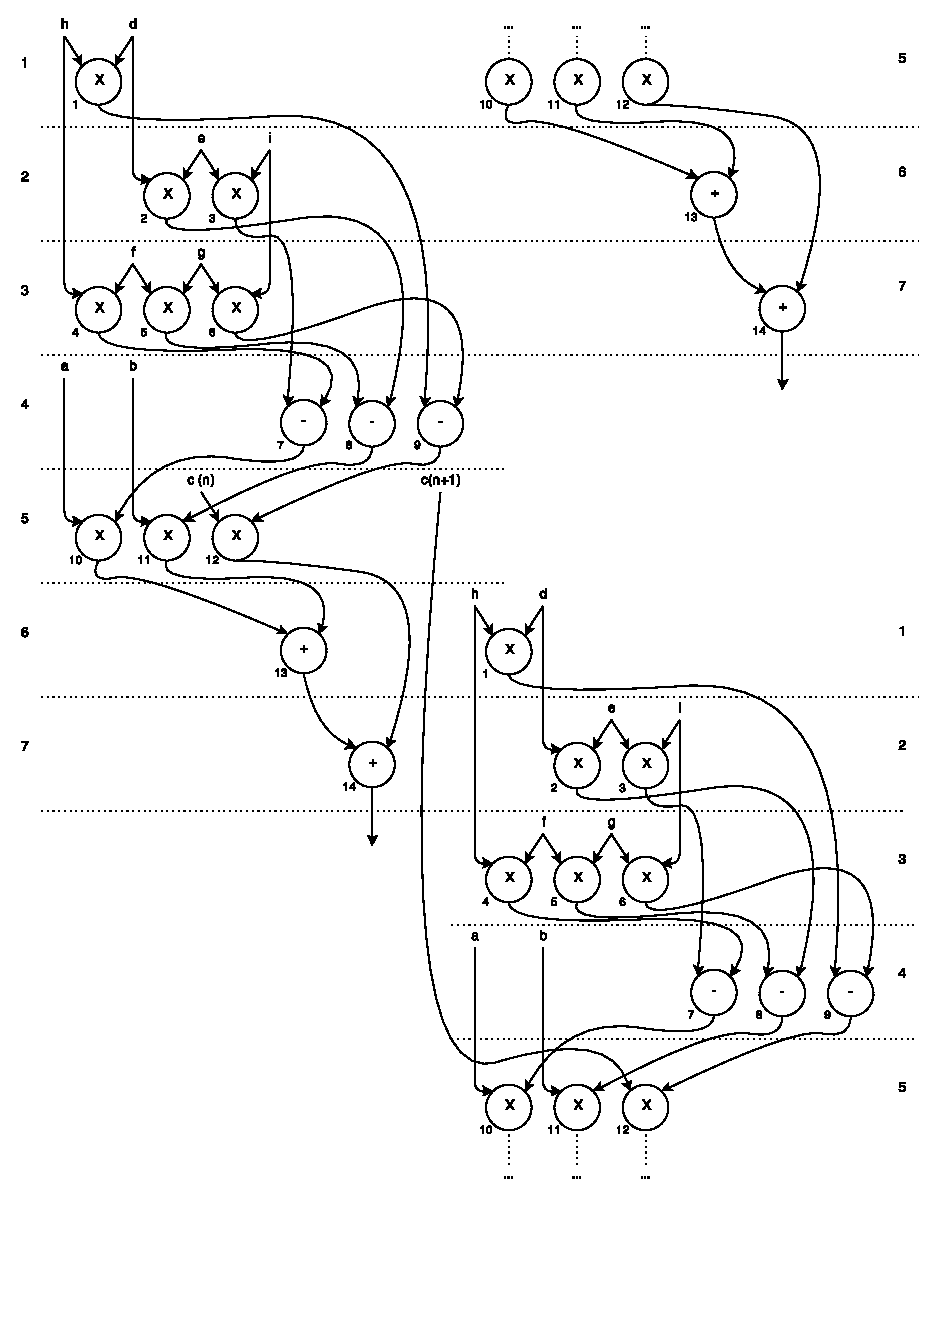
\includegraphics[width=0.7\paperwidth]{scheduling_2portRAM_maxthrough}}
\caption{Escalonamento para maximizar \textit{throughput}}
\label{fig:scheduling_2portRAM_maxthrough}
\end{figure}

Uma vez que o número de operandos a ler é ímpar ($9$), e como o objectivo é maximizar o \emph{throughput}, haverá dois tipos distintos de execução.

\noindent\rule{\linewidth}{0.4pt}

\begin{multicols}{2}

	\subsubsection{Execuções ímpares}

	\begin{table}[H]
		\centering
		\begin{tabular}{l|c|c}
			Operação & \multicolumn{2}{c}{Operandos} \\
			\hline
			\texttt{READ} & $d$ & $h$ \\
			\hline
			\texttt{MUL} & $d$ & $h$ \\
			\hline
			\texttt{STORE} & \multicolumn{2}{c}{$R_1\leftarrow d$} \\
			\texttt{STORE} & \multicolumn{2}{c}{$R_2\leftarrow h$} \\
			\texttt{STORE} & \multicolumn{2}{c}{$R_3\leftarrow dh$} \\
		\end{tabular}
		\caption{Operações do 1º ciclo de execução ímpar}
		\label{tab:odd_1}
	\end{table}

	\begin{table}[H]
		\centering
		\begin{tabular}{l|c|c}
			Operação & \multicolumn{2}{c}{Operandos} \\
			\hline
			\texttt{READ} & $i$ & $e$ \\
			\hline
			\texttt{MUL} & $i$ & $e$ \\
			\texttt{MUL} & $i$ & $R_1$($d$) \\
			\hline
			\texttt{STORE} & \multicolumn{2}{c}{$R_1\leftarrow di$} \\
			\texttt{STORE} & \multicolumn{2}{c}{$R_4\leftarrow e$} \\
			\texttt{STORE} & \multicolumn{2}{c}{$R_5\leftarrow ei$} \\
		\end{tabular}
		\caption{Operações do 2º ciclo de execução ímpar}
		\label{tab:odd_2}
	\end{table}

	\begin{table}[H]
		\centering
		\begin{tabular}{l|c|c}
			Operação & \multicolumn{2}{c}{Operandos} \\
			\hline
			\texttt{READ} & $f$ & $g$ \\
			\hline
			\texttt{MUL} & $f$ & $g$ \\
			\texttt{MUL} & $f$ & $R_2$($h$) \\
			\texttt{MUL} & $g$ & $R_4$($e$) \\
			\hline
			\texttt{STORE} & \multicolumn{2}{c}{$R_6\leftarrow fg$} \\
			\texttt{STORE} & \multicolumn{2}{c}{$R_2\leftarrow fh$} \\
			\texttt{STORE} & \multicolumn{2}{c}{$R_4\leftarrow eg$} \\
		\end{tabular}
		\caption{Operações do 3º ciclo de execução ímpar}
		\label{tab:odd_3}
	\end{table}

	\begin{table}[H]
		\centering
		\begin{tabular}{l|c|c}
			Operação & \multicolumn{2}{c}{Operandos} \\
			\hline
			\texttt{READ} & $a$ & $b$ \\
			\hline
			\texttt{SUB} & $R_5$($ei$) & $R_2$($fh$) \\
			\texttt{SUB} & $R_6$($fg$) & $R_1$($di$) \\
			\texttt{SUB} & $R_3$($dh$) & $R_4$($eg$) \\
			\hline
			\texttt{STORE} & \multicolumn{2}{c}{$R_1\leftarrow a$} \\
			\texttt{STORE} & \multicolumn{2}{c}{$R_2\leftarrow b$} \\
			\texttt{STORE} & \multicolumn{2}{c}{$R_4\leftarrow ei - fh$} \\
			\texttt{STORE} & \multicolumn{2}{c}{$R_5\leftarrow fg - di$} \\
			\texttt{STORE} & \multicolumn{2}{c}{$R_6\leftarrow dh - eg$} \\
		\end{tabular}
		\caption{Operações do 4º ciclo de execução ímpar}
		\label{tab:odd_4}
	\end{table}

	\begin{table}[H]
		\centering
		\begin{tabular}{l|c|c}
			Operação & \multicolumn{2}{c}{Operandos} \\
			\hline
			\texttt{READ} & $c$ & $c_{n+1}$ \\
			\hline
			\texttt{MUL} & $R_4$ & $R_1$ \\
			\texttt{MUL} & $R_5$ & $R_2$ \\
			\texttt{MUL} & $R_6$ & $c$ \\
			\hline
			\texttt{STORE} & \multicolumn{2}{c}{$R_4\leftarrow R_1R_4$} \\
			\texttt{STORE} & \multicolumn{2}{c}{$R_5\leftarrow R_2R_5$} \\
			\texttt{STORE} & \multicolumn{2}{c}{$R_6\leftarrow c R_6$} \\
			\texttt{STORE} & \multicolumn{2}{c}{$R_8\leftarrow c_{n+1}$} \\
		\end{tabular}
		\caption{Operações do 5º ciclo de execução ímpar}
		\label{tab:odd_5}
	\end{table}

	\begin{table}[H]
		\centering
		\begin{tabular}{l|c|c}
			Operação & \multicolumn{2}{c}{Operandos} \\
			\hline
			\texttt{ADD} & $R_4$ & $R_5$ \\
			\hline
			\texttt{STORE} &\multicolumn{2}{c}{$R_7\leftarrow R_4R_5$} \\
		\end{tabular}
		\caption{Operações do 6º ciclo de execução ímpar}
		\label{tab:odd_6}
	\end{table}

	\begin{table}[H]
		\centering
		\begin{tabular}{l|c|c}
			Operação & \multicolumn{2}{c}{Operandos} \\
			\hline
			\texttt{ADD} & $R_7$ & $R_6$ \\
			\hline
			\texttt{STORE} &\multicolumn{2}{c}{$R_7\leftarrow \left|\begin{matrix}a&b&c\\d&e&f\\g&h&i\end{matrix}\right|$} \\
		\end{tabular}
		\caption{Operações do 7º ciclo de execução ímpar}
		\label{tab:odd_7}
	\end{table}

	\subsubsection{Execuções pares}

	Os primeiros 4 ciclos de execução par são idênticos aos da execução ímpar (Ver Tabelas~\ref{tab:odd_1}-\ref{tab:odd_3}).

	\begin{table}[H]
		\centering
		\begin{tabular}{l|c|c}
			Operação & \multicolumn{2}{c}{Operandos} \\
			\hline
			\texttt{MUL} & $R_4$ & $R_1$ \\
			\texttt{MUL} & $R_5$ & $R_2$ \\
			\texttt{MUL} & $R_6$ & $R_8$ \\
			\hline
			\texttt{STORE} & \multicolumn{2}{c}{$R_4\leftarrow R_1R_4$} \\
			\texttt{STORE} & \multicolumn{2}{c}{$R_5\leftarrow R_2R_5$} \\
			\texttt{STORE} & \multicolumn{2}{c}{$R_6\leftarrow R_3R_6$} \\
		\end{tabular}
		\caption{Operações do 5º ciclo de execução par}
		\label{tab:even_5}
	\end{table}

	Igualmente, os ciclos 6 e 7 são idênticos em termos de operações aos das execuções ímpares (Ver Tabelas~\ref{tab:odd_6}~e~\ref{tab:odd_7}).

\end{multicols}
\noindent\rule{\linewidth}{0.4pt}


\subsubsection{Diagrama de Execuções}

\begin{figure}[H]
	\centering
	\begin{tabular}{|l||c|c|c|c|c|c|c|c|c|c|c|c|}
		\hline
		Execução $n$ & 1 & 2 & 3 & 4 & 5 & 6 & 7 &&&&&\\
		\hline
		Execução $n+1$ &&&&&& 1 & 2 & 3 & 4 & 5 & 6 & 7 \\
		\hline
		Execução $n+2$ &&&&&&&&&& 1 & 2 & 3 \\
		\hline
	\end{tabular}
	\caption{Diagrama de Execuções para $n$ ímpar}
	\label{fig:datapath_max_throughput}
\end{figure}

Com este tipo de execução, o número total de ciclos para processar 100 conjuntos de dados é:

\[ \frac{100}{2} \cdot 5 + \frac{100}{2} \cdot 4 + 3 = \]
\[= 250 + 200 + 3 =\]
\[= 453\]
